The TUPT package is a package in active development.
Its main purpose is to (a) scan a site for metadata, (b) correct metadata and (c) find resources corresponding
to this corrected metadata.
The current implementation of TUPT is aimed at movies, with the resource collection being done
through torrent sites.
The main activity diagram for this functionality can be found in \autoref{fig:activitytupt}.
The general package class diagram for the TUPT project can be found in \autoref{fig:classdiagramgeneraltupt}.
The specific top-level TUPT package classes class diagram can be found in \autoref{fig:classdiagramspecifictupt}.
The main entrypoint for the package is the TUPTControl class.
The process of the aforementioned TUPT chain goes through 4 sub-packages, in order these are:
the Parser, the Matcher, the TorrentFinder and then the Channels sub-package.

First a webpage is parsed for possible movies by the Parser package (for class diagram see \autoref{fig:classdiagramparser}).
Given an URL the Parser control class will query its plug-ins whether they can parse the website.
If they can, they are queried to process the raw html of the website and return none or more 
found movies (in the form of Movie classes).
The main entrypoint for the sub-package is the ParserControl class.

Secondly this (possibly very minimal) movie metadata will be corrected and supplemented.
This is done by the Matcher package, see \autoref{fig:activitymatcher} for the activity diagram
of how different results from different plugins are bound together to correct the metadata.
The class diagram of this sub-package is shown in \autoref{fig:classdiagrammatcher}.
The main entrypoint for the sub-package is the MatcherControl class.

Thirdly this corrected movie metadata is used to find a corresponding torrent file in the TorrentFinder sub-package.
Plug-ins are queried to produce .torrent-file links and/or magnet links for the given movie metadata,
see \autoref{fig:activitytorrentfinder} for the activity diagram of this function.
The class diagram of this sub-package is shown in \autoref{fig:classdiagramtorrentfinder}.
The main entrypoint for the sub-package is the TorrentFinderControl class.

Lastly the corrected movie metadata coupled to the best torrent file that could be found
and inserted cleanly into a user's Tribler channel.
The class diagram for this Channels sub-package is given in \autoref{fig:classdiagramchannels}.
The main entrypoint for the sub-package is the MovieInserter class.

\begin{figure}[hp]
  \centering
      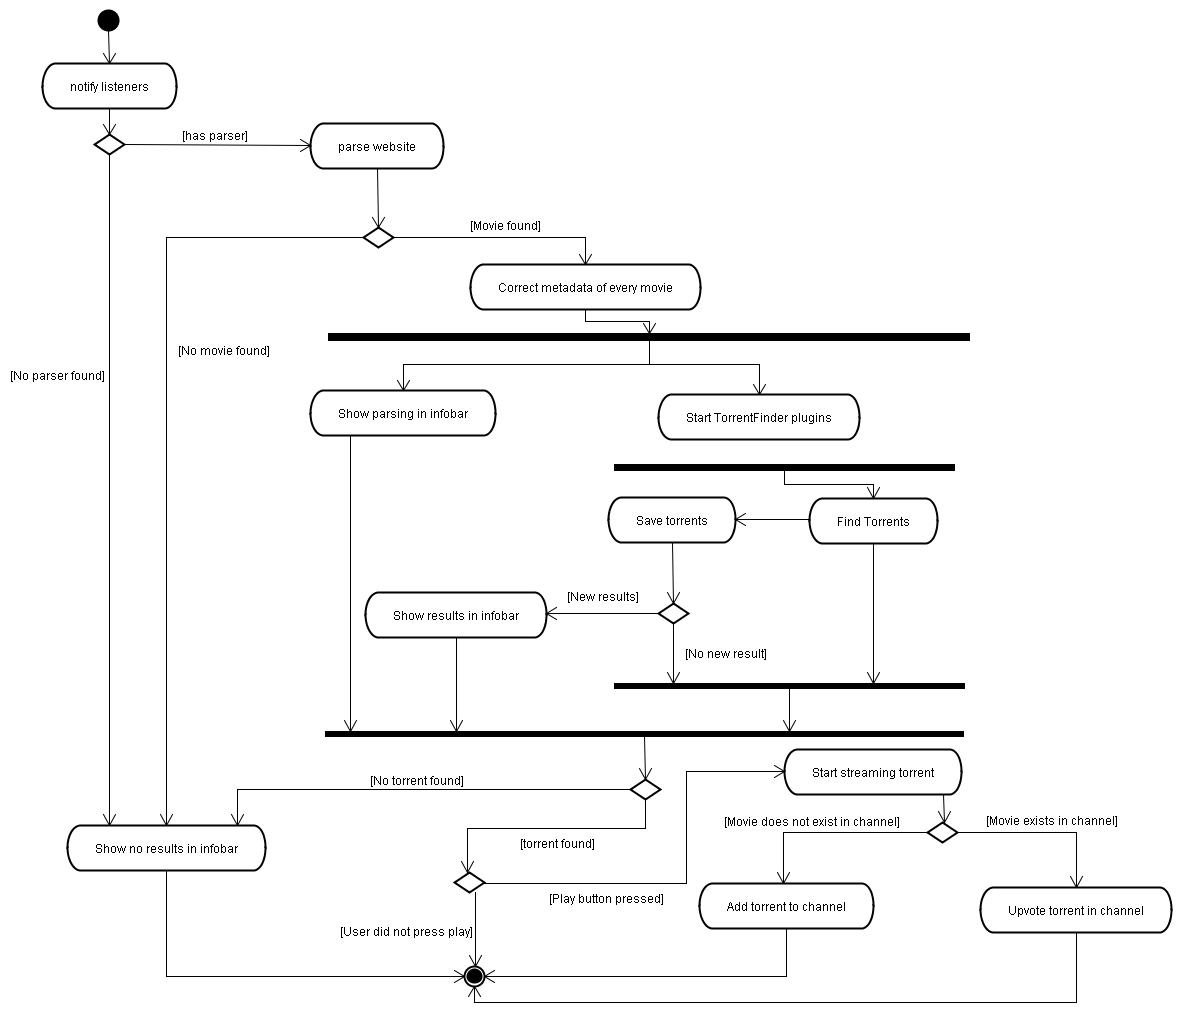
\includegraphics[width=0.8\textwidth]{TUPT-activitydiagram.jpg}
  \caption{Activity diagram of general TUPT functionality}
  \label{fig:activitytupt}
\end{figure}

\begin{figure}[hp]
  \centering
\tikzimgGeneralTUPT
  \caption{Class diagram for the entire TUPT package}
  \label{fig:classdiagramgeneraltupt}
\end{figure}

\begin{figure}[hp]
  \centering
\tikzimgSpecificTUPT
  \caption{Class diagram for the top-level TUPT package}
  \label{fig:classdiagramspecifictupt}
\end{figure}

\begin{figure}[hp]
  \centering
\tikzimgParser
  \caption{Class diagram for the Parser sub-package}
  \label{fig:classdiagramparser}
\end{figure}

\begin{figure}[hp]
  \centering
      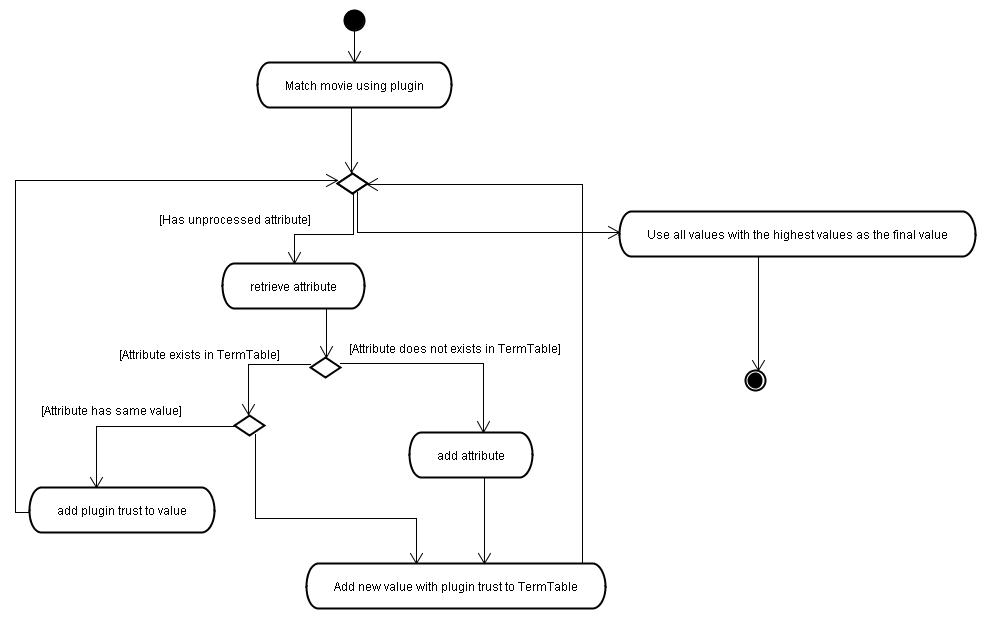
\includegraphics[width=0.8\textwidth]{Matcher-activitydiagram.jpg}
  \caption{Activity diagram of the Matcher sub-package}
  \label{fig:activitymatcher}
\end{figure}

\begin{figure}[hp]
  \centering
\tikzimgMatcher
  \caption{Class diagram for the Matcher sub-package}
  \label{fig:classdiagrammatcher}
\end{figure}

\begin{figure}[hp]
  \centering
      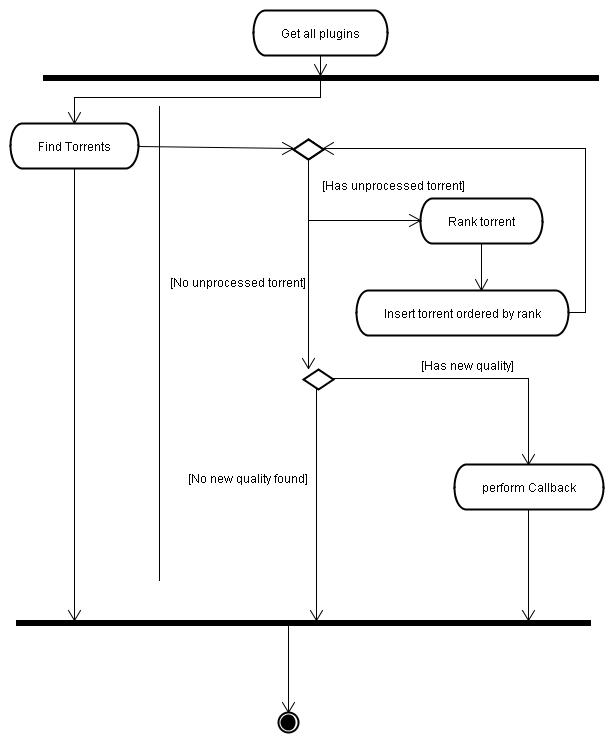
\includegraphics[width=0.8\textwidth]{TorrentFinder-activitydiagram.jpg}
  \caption{Activity diagram of the TorrentFinder sub-package}
  \label{fig:activitytorrentfinder}
\end{figure}

\begin{figure}[hp]
  \centering
\tikzimgTorrentFinder
  \caption{Class diagram for the TorrentFinder sub-package}
  \label{fig:classdiagramtorrentfinder}
\end{figure}

\begin{figure}[hp]
  \centering
\tikzimgChannels
  \caption{Class diagram for the Channels sub-package}
  \label{fig:classdiagramchannels}
\end{figure}